\chapter{Results}\label{chapter:results}
%Tables
%charts
\section{Sample applications made using the framework}

\section{Benchmarks}
The benchmark results illustrated in this chapter were performed on Amazon EC2 server\footnote{EC2 servers of Frankfurt data center} with configurations shown in table~\autoref{tab:specs}

\begin{table}[htsb]
  \caption[Specification of machines used for testing and benchmarking]{Specification of machines used for testing and benchmarking}\label{tab:specs}
  \centering
  \begin{tabular}{l l l}
    \toprule
      Deployed Systems & Name &  Specifications\\
    \midrule

      \pbox{30cm}{\relax RabbitMQ and\\a Message Queuing System} & c3.2xLarge & \pbox{60cm}{8 core CPU, 28 ECU,\\15 GiB Memory, SSD disk}\\
\midrule
      \pbox{30cm}{\relax Message Queuing System} & m3.2xLarge & \pbox{60cm}{8 core CPU, 26 ECU,\\30 GiB Memory, SSD disk}\\
\midrule
      \pbox{20cm}{\relax Registry} & m3.xLarge & \pbox{60cm}{2 core CPU, 13 ECU,\\15 GiB Memory, SSD disk}\\
\midrule
      \pbox{20cm}{\relax Isolate Systems (Nodes)} & m3.xLarge & \pbox{60cm}{2 core CPU, 13 ECU,\\15 GiB Memory, SSD disk}\\

    \bottomrule
  \end{tabular}
\end{table}

\subsection{Prefetch Count}
\autoref{fig:result-prefetch} shows the variation in overall message consumption when the number of consumers (separate isolate systems in separate nodes) were increased. Each line in the figure represents different values of prefetch-count set in the consumer while subscribing to the message broker system. Depending upon prefetch-count, saturation point and decrease rate can also be seen when number of consumers were increased.

  The increase in consumers had significant positive result for message throughput, but we can see that after around 8 consumers, adding more consumers had negative effect in the overall throughput.

    Increasing prefetch count had more positive impact in message throughput compared to increasing consumers. For instance, increase in consumers from 1 to 16 resulted in the rise of approximately 2000 message per second, while the increase in prefetch count from 1 to 16 in single consumer resulted in increase of message throughput by approximately 5500 messages per second.

\begin{figure}[H]
  \centering
  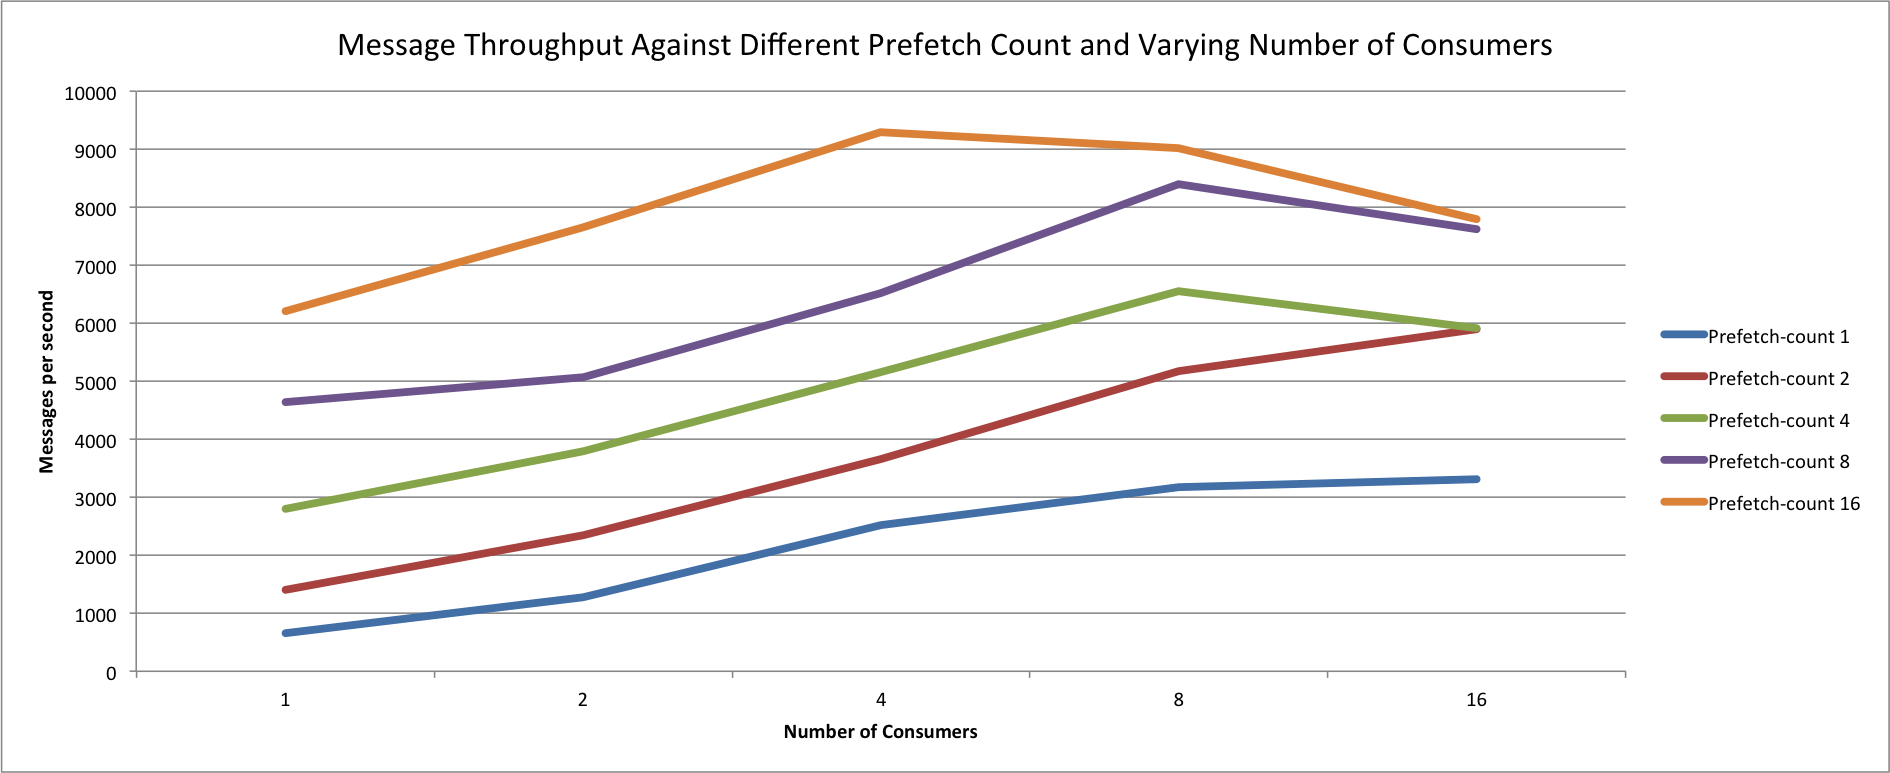
\includegraphics[width=1\textwidth]{figures/01prefetch}
  \caption[Message Throughput vs Number of consumers for varying prefetch-count]{Message Throughput vs Number of consumers for varying prefetch-count (Higher is better)}
  \label{fig:result-prefetch}
\end{figure}

\subsection{Message Size}
The result shown in \autoref{fig:result-consumptionMessageSize} was obtained by allowing eight consumers with the prefetch count of 8 to dequeue existing messages from a queue.

  The negative effect, on message consumption throughput, of larger message is evident from the  \autoref{fig:result-consumptionMessageSize}. The decrease in message throughput was more prominent between message size of 256 bytes and 512 bytes than that of between 64 bytes and 256 bytes.

  Similar observation can be made from~\autoref{fig:result-productionMessageSize} which is a result of allowing a single worker isolate to create messages, except there is slight rise in the throughput when the message size was increase from 512 bytes to 1024 bytes.

\begin{figure}[H]
  \centering  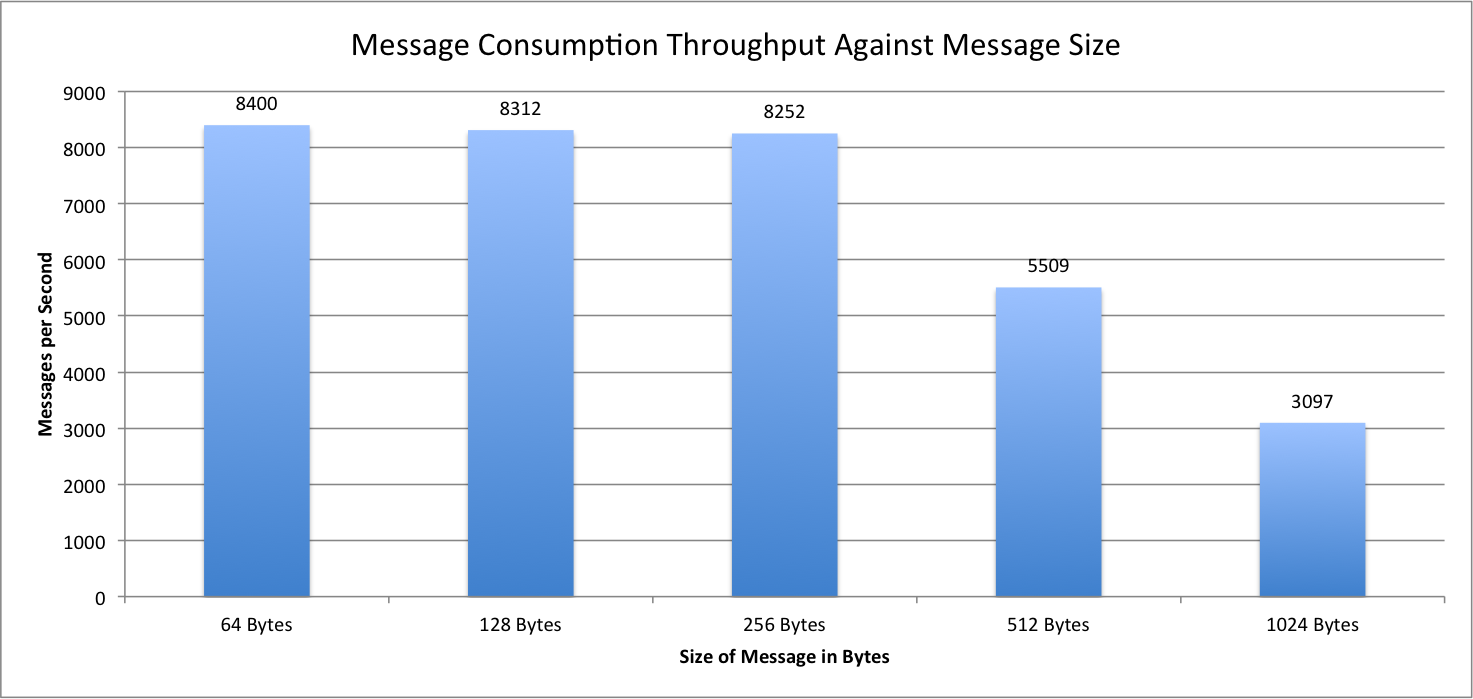
\includegraphics[width=1\textwidth]{figures/02consumptionMessageSize}
  \caption[Message Consumption Throughput vs Message Size]{Message Consumption Throughput vs Message Size (Higher is better)}
  \label{fig:result-consumptionMessageSize}
\end{figure}

\begin{figure}[H]
  \centering  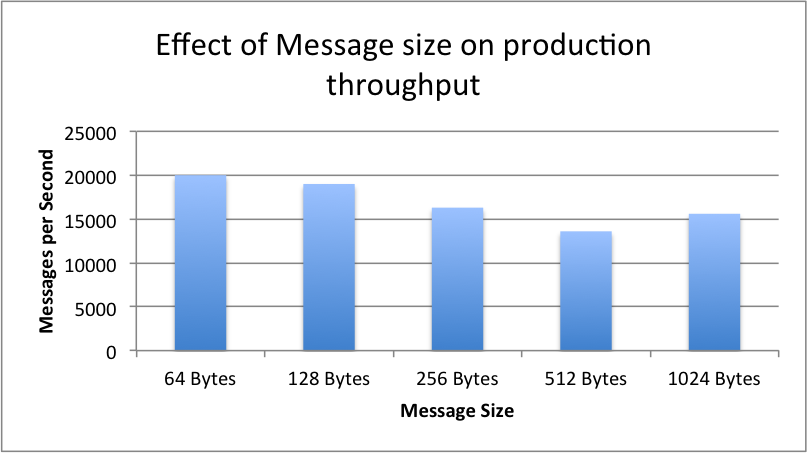
\includegraphics[width=0.8\textwidth]{figures/03productionMessageSize}
  \caption[Message Production Throughput vs Message Size]{Message Production Throughput vs Message Size (Higher is better)}
  \label{fig:result-productionMessageSize}
\end{figure}

\subsection{Number of Message Queuing Systems}

\begin{figure}[H]
  \centering
  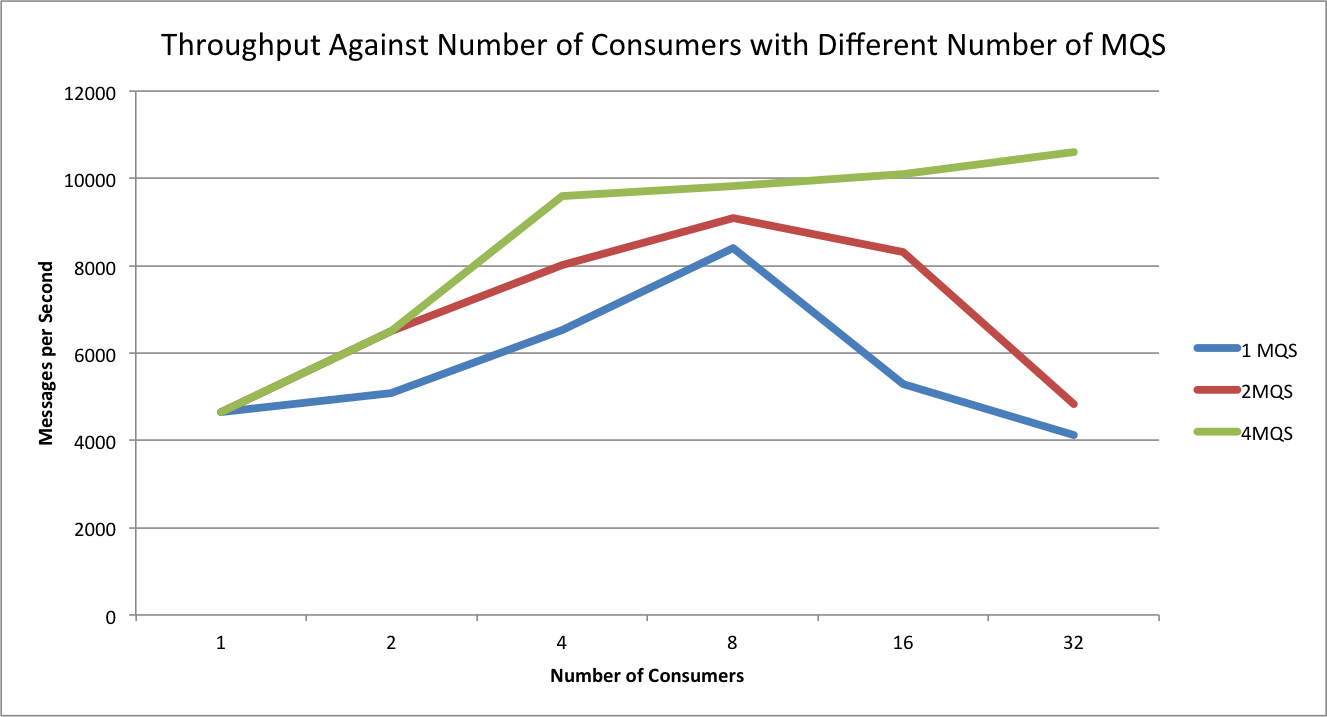
\includegraphics[width=1\textwidth]{figures/04varyingMqs}
  \label{fig:result-varyingMqs}
\end{figure}


\begin{figure}[H]
  \centering
  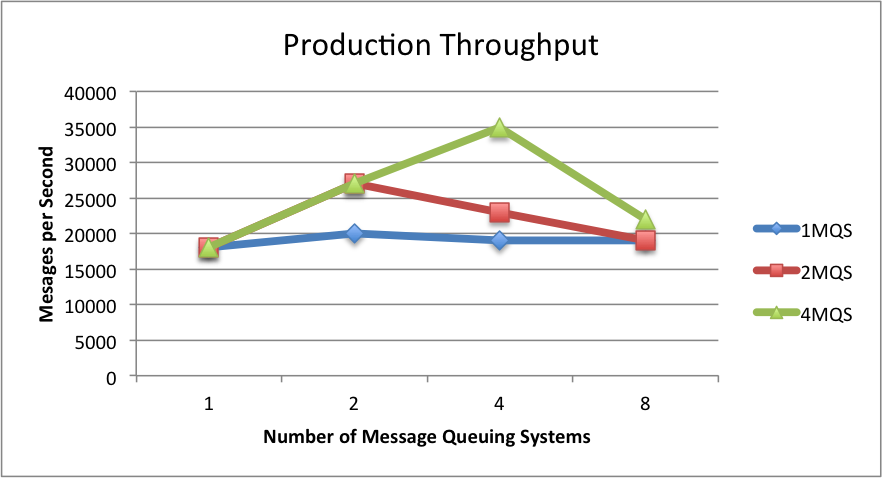
\includegraphics[width=1\textwidth]{figures/05productionRabbit}
  \label{fig:result-productionRabbit}
\end{figure}


\begin{figure}[H]
  \centering
  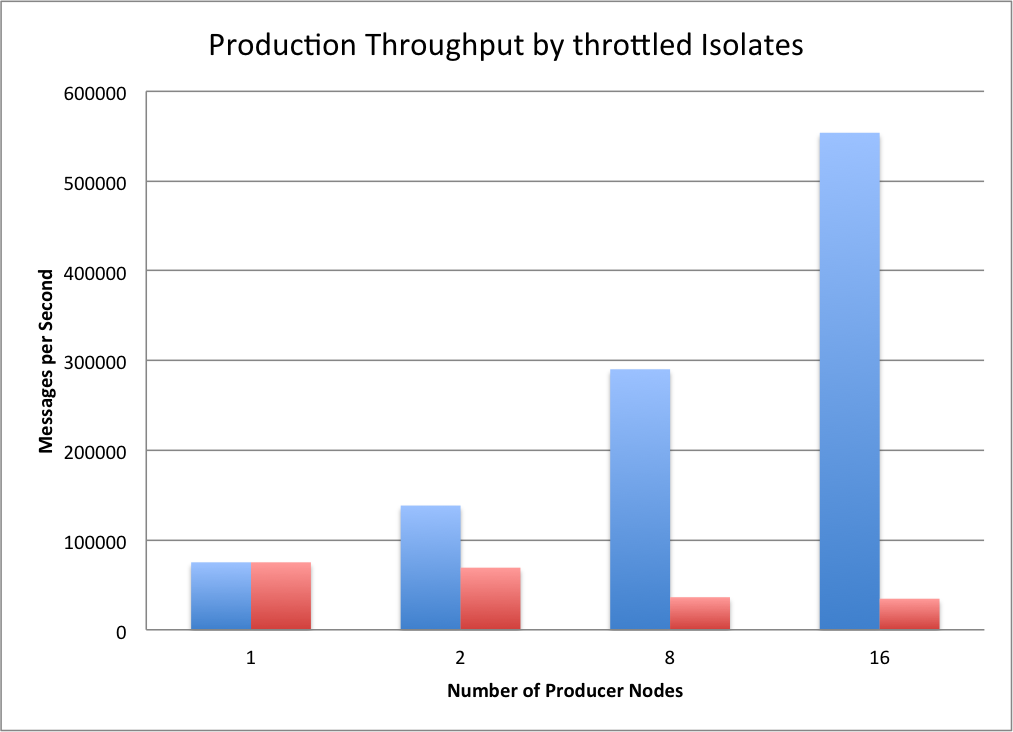
\includegraphics[width=1\textwidth]{figures/06productionIsolate}
  \label{fig:result-productionIsolate}
\end{figure}


\begin{figure}[H]
  \centering
  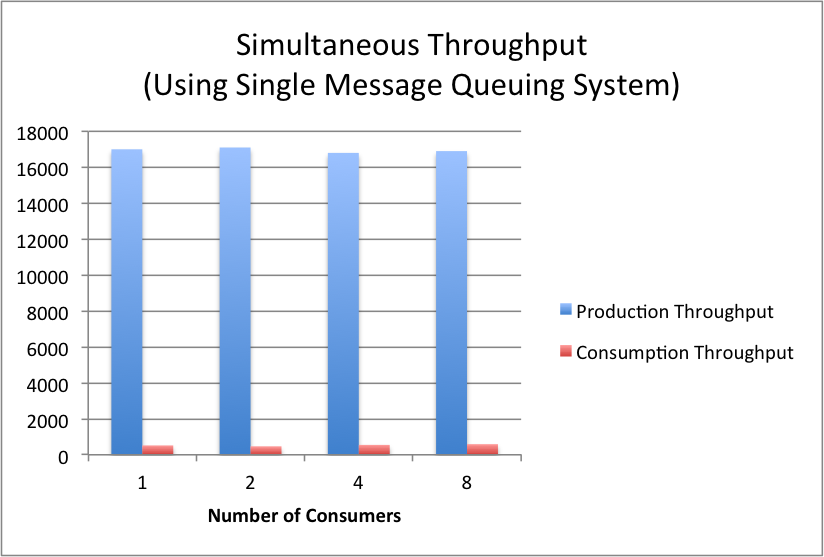
\includegraphics[width=1\textwidth]{figures/07simultaneous1}
  \label{fig:result-simultaneous1}
\end{figure}


\begin{figure}[H]
  \centering
  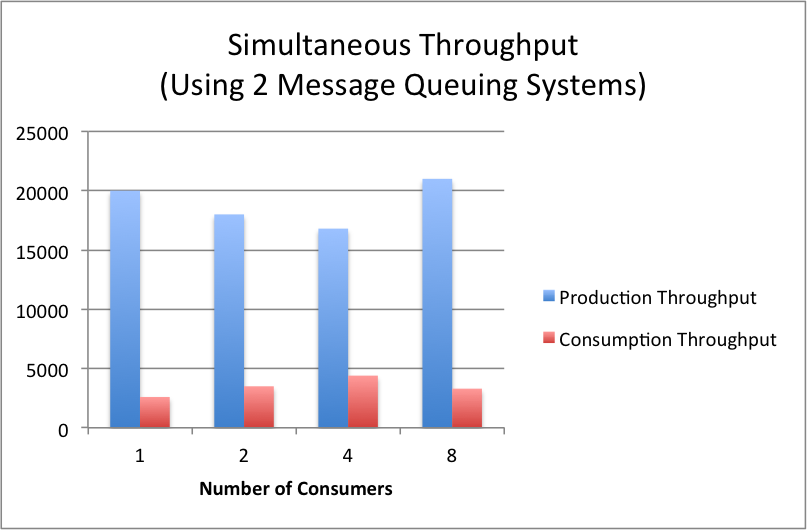
\includegraphics[width=1\textwidth]{figures/08simultaneous2}
  \label{fig:result-simultaneous2}
\end{figure}


\begin{figure}[H]
  \centering
  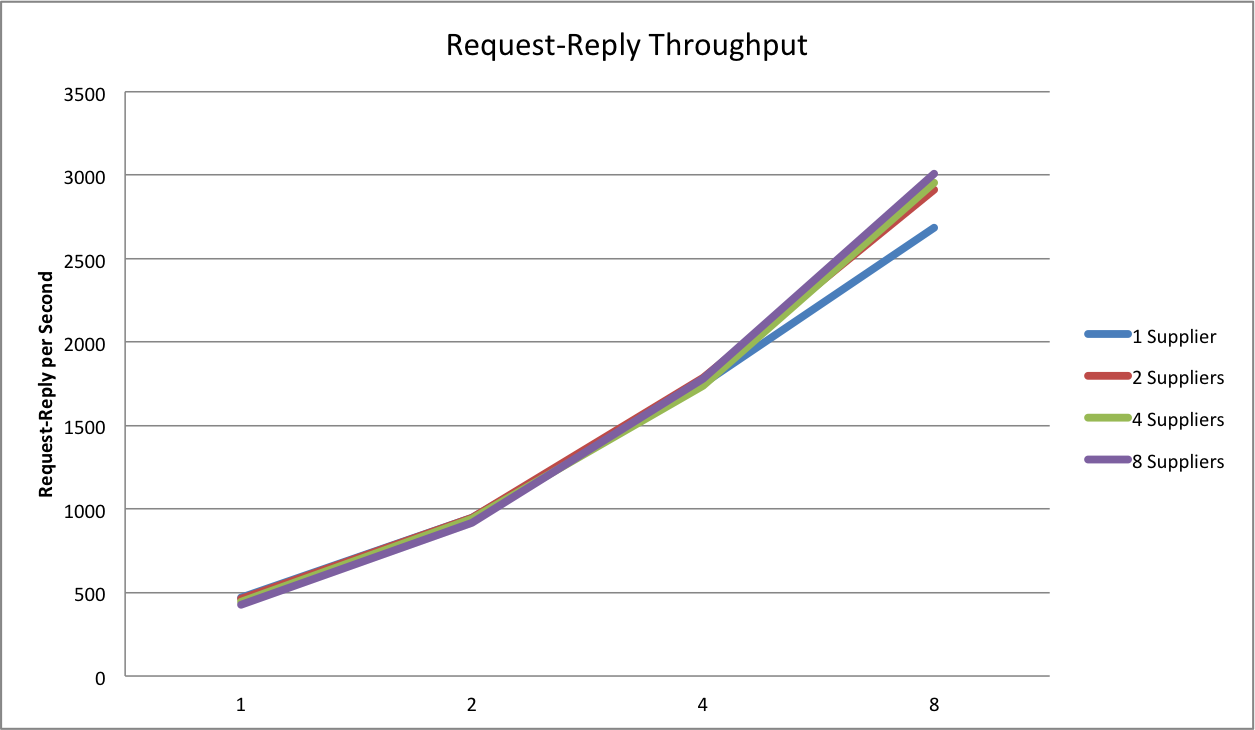
\includegraphics[width=1\textwidth]{figures/09request-reply}
  \label{fig:result-request-reply}
\end{figure}
